The \dword{larasic} receives signals from the CR board and
provides a means to amplify and shape the current signals originally coming from the TPC wires; the
shaping serves as an anti-aliasing filter for the TPC signals.
Each \dword{larasic} channel has a charge amplifier circuit with a programmable
gain selectable from one of \num{4.7}, \num{7.8}, \num{14} or \SI{25}{mV/fC}
(corresponding to full-scale charge of \num{300}, \num{180}, \num{100} and \SI{55}{fC}),
a high-order anti-aliasing filter with programmable time
constant (semi-Gaussian with peaking time \num{0.5}, \num{1}, \num{2}, and \SI{3}{\micro\second}),
an option to enable AC coupling,
and a baseline adjustment for operation with either the collecting (\SI{200}{mV} nominal) or the non-collecting (\SI{900}{mV} nominal) wires.

Figure~\ref{fig:fe-output} (left) shows the simulated pulse response for all gains and peaking times and both baselines.
Note that the gain is independent of the peaking time;  the same amount of charge produces the same peak voltage signal regardless of the peaking time.  

Shared among the \num{16} channels in the \dword{larasic} are the bias circuits, programming registers,
a temperature monitor, an analog buffer for signal monitoring, and the digital interface.
The power dissipation of \dword{larasic} is about \SI{6}{mW} per channel at \SI{1.8}{V} supply voltage.

The \dword{larasic} is implemented using the TSMC \SI{180}{nm} \dword{cmos} process.\footnote{TSMC 0.18-micron Technology\texttrademark{}, Taiwan Semiconductor Manufacturing Company Ltd., \url{http://www.tsmc.com/english/dedicatedFoundry/technology/0.18um.htm}.}  The charge sensitive amplifier uses a very large p-channel field effect transistor (PFET) with a width of \SI{20}{mm} and a length of \SI{270}{nm} followed by a dual cascode stage, a pulse shaping network, and a baseline restoration circuit.  

Each channel also implements a high-performance output driver 
that can be used to drive a long cable, but which is disabled when interfaced to an \dword{adc} \dword{asic} to reduce the power consumption.
The \dword{asic} integrates a band-gap reference (BGR) to generate all the internal bias voltages and currents.
This guarantees a high stability of the operating point over a wide range of
temperatures, including cryogenic temperatures.
The \dword{asic} is packaged in a commercial, fully encapsulated plastic QFP~80 package.

\begin{dunefigure}
[Simulated \dword{fe} response to an instantaneous injected charge]
{fig:fe-output}
{Simulated \dword{fe} response to an instantaneous injected charge for all gains and peaking times and both baselines (left); also shown are measured calibration pulse response overlays for \num{2560} electronics channels (baseline subtracted) attached to a \dword{pdsp} \dword{apa} (right).  Note that the truncated negative pulses are due to effects of saturation associated with the collection plane threshold being close to the lower \dword{adc} boundary.}
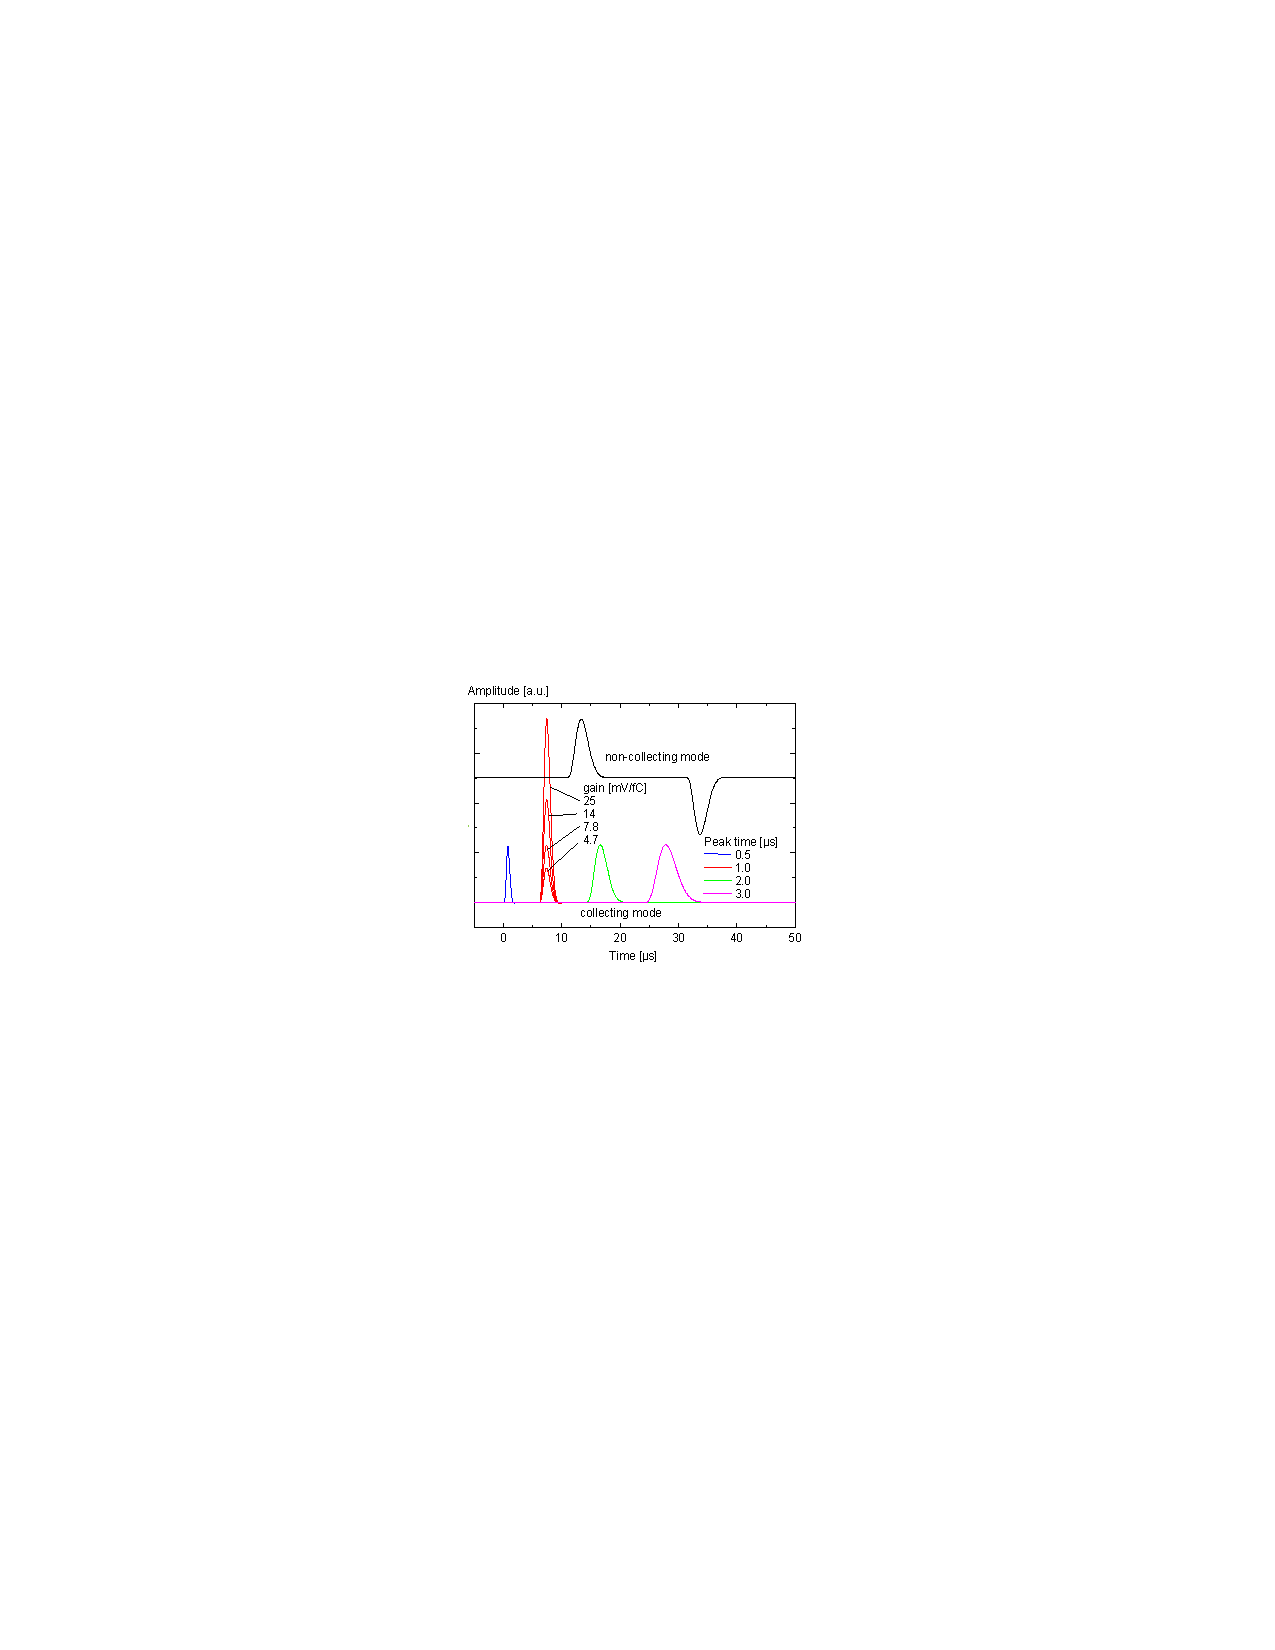
\includegraphics[width=0.47\linewidth]{tpcelec-shaper_out.pdf}
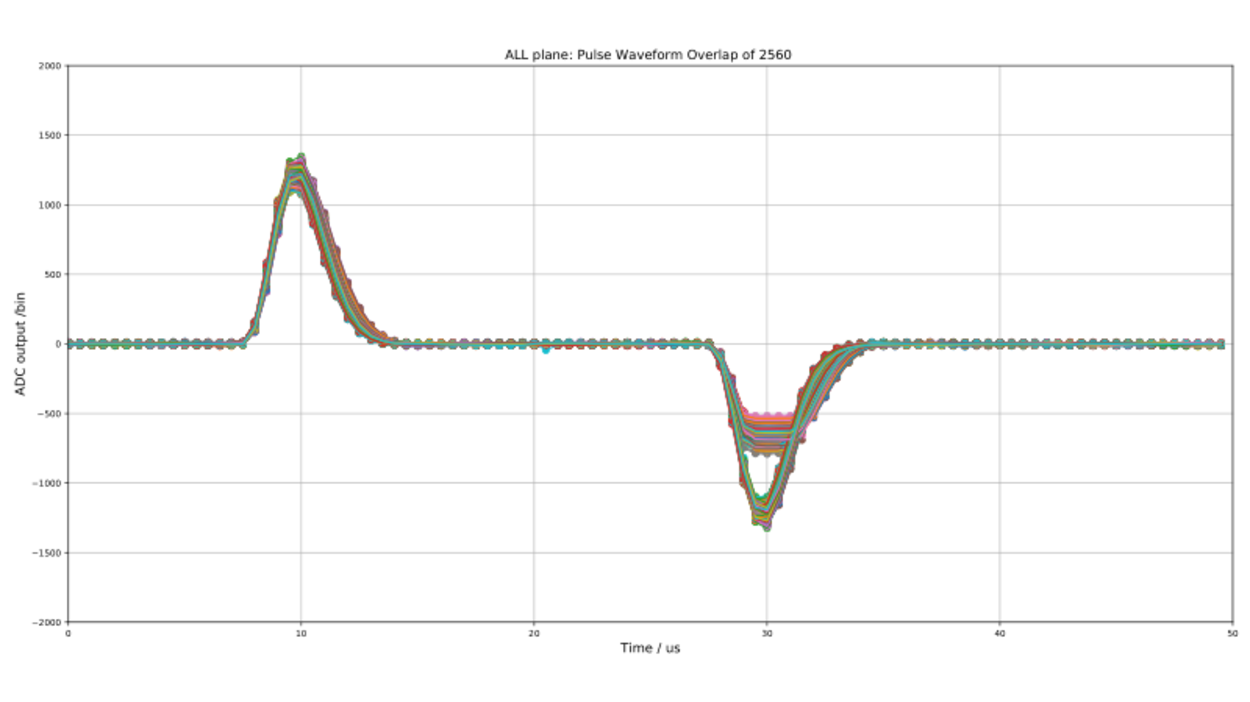
\includegraphics[width=0.5\linewidth]{tpcelec-pdune-wf.pdf}
\end{dunefigure}

Each \dword{fe} \dword{larasic} channel is equipped with an injection capacitor which can be used
for test and calibration and can be enabled or disabled through a
dedicated register. The injection capacitance has been measured to \num{0.5}\% using 
a calibrated external capacitor. The measurements show
that the calibration capacitance is extremely stable, changing from
\SI{184}{fF} at room temperature to \SI{183}{fF} at \SI{77}{K}. This result and the measured
stability of the peaking time demonstrate the high stability of the
passive components as a function of temperature. Channel-to-channel and chip-to-chip
variation in the calibration capacitor are typically less than \num{1}\%. 

Prototype \dwords{larasic} have been evaluated and characterized at room temperature and LN 
(\SI{77}{K}) temperature.
During testing the circuits have been cycled multiple times
between the two temperatures and operated without any change in performance.
Figure~\ref{fig:fe-output} (right) shows the measured injection pulse response overlaid with the baseline subtracted for one full \dword{apa} 
(\num{2560}) electronics channels from \dword{pdsp} \dword{femb} attached to a \dword{pdsp} \dword{apa} in a 
shielded environment at approximately \SI{180}{K}. This contains \num{1600} induction (high-baseline)
and \num{960} collection (low-baseline) channels, the latter of which saturate the negative pulse at the low 
end of the \dword{fe} output. The spread in saturization values between \num{-500} and \num{-750} \dword{adc} bins is due to the
variation in relative position of the \dword{fe} baseline to the low end of the \dword{fe} output 
in the \dword{pdsp} version of the \dword{larasic}.
%These results are in close agreement with simulations and indicate
%that both the analog and the digital circuits and interface operate as
%expected in a cryogenic environment.



